\documentclass[a4paper]{article}
\usepackage[utf8]{inputenc}
\usepackage[T2A]{fontenc}
\usepackage[english,russian]{babel}
\usepackage[left=25mm, top=20mm, right=25mm, bottom=20mm, nohead]{geometry}
\usepackage{amsmath, amsfonts, amssymb}
\usepackage{graphicx} 
\newcommand{\lrl}[1]{\({#1}\)}
\graphicspath{{./images/}}

\title{\vspace{-2cm}Graphs SGA}
\author{Andrey Baranov}
\date{May 2023}

\begin{document}


\maketitle
\subsection*{1.}
In a country there are several airports. Airport \(A\) is directly connected to 23 other airports. Airport \(B\) has a direct connection to 3 other airports. Each airport, except \(A\) and \(B\), is directly connected to 10 other airports. Prove that there is an airline route (maybe with flight changes) between \(A\) and \(B\).
\subsubsection*{Solution}
\par To prove that there is an airline route between airport A and airport B, we can use a concept in graph theory called \textbf{connectedness}. In this case, we can represent the airports as \textit{vertices} on a graph, and the direct connections between them as \textit{edges}. The graph is considered \textbf{connected} if and only if every \textit{vertex} \(X\) of the graph can be reached from any \textit{vertex} \(Y\) through one or more \textit{edges} of the graph. \\
\par
First, we know that airport \(A\) is directly connected to 23 other airports, so we can draw a \textit{vertex} for airport \(A\) and connect it to 23 other vertices. Similarly, we can draw a \textit{vertex} for airport \(B\) and connect it to 3 other vertices. \\
\par
For all other airports (not \(A\) or \(B\)), we know that each is directly connected to 10 other airports. So we can draw \textit{vertices} for each of these airports and connect them to 10 other vertices. \\
\par
Now we have a graph where all vertices represent airports, and the edges represent direct connections between them, it still might be difficult to determine if there is a path between A and B just by looking at the graph.
But we can use the concept of \textbf{connectedness}. A graph is considered "connected" if there is a path between any two vertices. If a graph is not connected, it is made up of smaller \textbf{components} that are connected. \\
\par
In this case, we know that airport \(A\) is directly connected to 23 other airports, and each of those airports is directly connected to 10 other airports. So we can imagine that this creates a large \textit{component} of the graph that is connected to airport \(A\). \\
\par
Similarly, airport \(B\) is directly connected to 3 other airports, and each of those airports is directly connected to 10 other airports. This creates another \textit{component} of the graph that is connected to airport \(B\). \\
\par
Now we just need to show that these two components are connected to each other. This can be done by finding a path between any \textit{vertex} in the component connected to \(A\) and any \textit{vertex} in the component connected to \(B\). We know that the two components must overlap at some airports, because there are other airports that are connected to both A and B (the ones that are directly connected to 10 other airports). \\
\par
Also we can prove this using handshaking lemma. Assume that airports \(A\) and \(B\), having 23 and 3 connected airports accordingly, are in different connected components. And all the other airports, except for \(A\) and \(B\), are connected to 10 others. Thus, each of this components violates the handshaking lemma, having exactly one odd vertex. \\
\par
So we can conclude that there is an airline route (maybe with flight changes) between airport \(A\) and airport \(B\), because the graph representing the airports and their direct connections is connected. \\
\subsection*{2.}
Consider an Erdős–Rényi random graph on 4 vertices with \(p=\frac{1}{2}\). Calculate the probability that this graph is connected.
\subsubsection*{Solution}
For an Erdős–Rényi random graph on 4 vertices with probability P = 1/2, we can use the probability formula to calculate the probability of having a certain number of edges:
\[
P(X=M) = p^M(1-p)^{\binom{n}{2}-M}
\]
where X is the random variable representing the number of edges \(M\), \(n\) is the total number of vertices, \(p\) is the probability of an edge being included, and \(\binom{n}{2}\)is the binomial coefficient. \\

\par In this case, \(n = 4\) (since there are 4 vertices), \(p = \frac{1}{2}\), and we can calculate the probability for each possible number of edges:
\[
P(0) = \frac{1}{2}^0(1-\frac{1}{2})^{\binom{4}{2}-0} = \frac{1}{64}
\]
\[
P(1) = \frac{1}{2}^1(1-\frac{1}{2})^{\binom{4}{2}-1} = \frac{1}{64}
\]
\[
P(2) = \frac{1}{2}^2(1-\frac{1}{2})^{\binom{4}{2}-1} = \frac{1}{64}
\]
\[
...
\] \\
\par Meaning with the probability \(p=\frac{1}{2}\) all the graphs on \(n\) vertices are chosen with equal probability in terms of Erdős–Rényi model.
We are interested only in cases when the number of edges in the graph are less than \(n-1=4-1=3\). That way such graph couldn’t be at least a tree to be connected. We can find the probability of a graph being connected by subtracting the sum of the probabilities of those graphs events from 1. \\
\par Maximum number of edges, for a graph on 4 vertices, to choose from is \(\frac{n(n-1)}{2}=\frac{4(4-1)}{2}=6\) in case of a complete graph. Let's start to calculate probabilities. For the case of a graph having 0 edges, there is only one such graph, meaning \(P(0) = \binom{6}{0} * \frac{1}{64}=\frac{1}{64}\). In the case of a graph having 1 edge, we can choose the place \(\binom{6}{1}\) different ways, having \(P(1)=\binom{6}{1}*\frac{1}{64}=\frac{6}{64}\). And the case to place 2 edges is \(P(2)=\binom{6}{2}*\frac{1}{64}=\frac{15}{64}\). As for the case of 3 edges, yes, this number of edges is minimum for the graph to be connected, but also, 3 is the maximum number of edges for the complete graph on 3 vertices, meaning we have 4 cases for each vertex to be isolated, of all the cases \(\binom{6}{3}=20\). Leaving us with the probability of the graph being disconnected on 4 vertices \(P(4) = 4 * \frac{1}{64}=\frac{4}{64}\). \\
\par Let's calculate the probability of the graph being connected as the opposite event, meaning:
\[
P(\textit{graph connected}) = 1 - \left(\frac{1}{64} +\frac{6}{64} + \frac{15}{64}+\frac{4}{64}\right)=\frac{38}{64}=\frac{19}{32}.
\]
\subsection*{3.}
Which of the following pictures can be drawn in one stroke of pen, without traversing a line twice (like a Euler path in a graph)?
\begin{center}
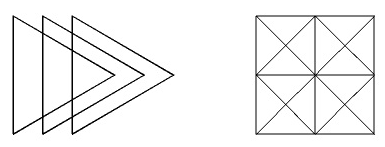
\includegraphics{task3.png}    
\end{center}
\subsubsection*{Solution}
Consider the left picture. Let's mark every interconnection between edges of the figure as vertices. After that, write down the degree for every vertex, having:
\begin{center}
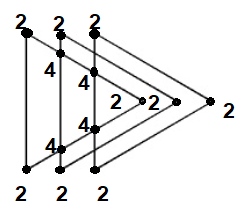
\includegraphics{task3_1.png}  
\end{center}
\par To find out if the considered figure could be drawn with one stroke of the pen is exactly to find an Eulerian path — such a path in a graph for which no edge traversed twice. To have an Eulerian path, one of two conditions must be satisfied. The graph should have an Eulerian cycle, meaning no vertex should have an odd degree. Or only two vertices in the graph gave an odd degree, meaning such a graph has an Eulerian trail. In the graph above, the first condition stands. Let's try to find an Eulerian path here:
\begin{center}
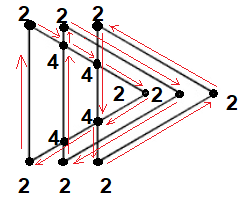
\includegraphics{task3_2.png}  
\end{center}
The graph above indeed has an Eulerian path. Thus, we have proven that this figure could be drawn with one stroke of a pen. \\

\par Now let's consider the right figure. Do the same, mark interconnections as edges, here we try to minimize the number of vertices. And afterwards, mark the degrees of those vertices. In any case of vertices here, since the figure is symmetric, we shall have a similar situation for the odd degree number. It is shown in the picture below: 
\begin{center}
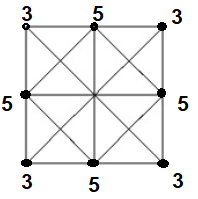
\includegraphics{task3_3.png}  
\end{center}
That way, for the case of the right figure, it is not possible to draw it with one stroke of a pen since the graph does not have an Eulerian path.
\subsection*{4.}
Does there exist a graph with 5 vertices which have the following degrees: 2, 4, 4, 4, 4?

\subsubsection*{Solution}
According to the Handshaking Lemma:
\[
\sum_{v\in{V}} deg\,v = 2|E|,
\]
where \(V\) is the set of vertices in the graph and \(E\) is the set of edges in the graph. We could substitute given values in the formula, having:
\[
2 + 4 + 4 + 4 + 4 = 18 = 2|E| \Rightarrow |E| = 9
\]
It seems like the condition stands. The sum of the vertices degrees is an even number, while the edge number is odd. The maximum number of edges in the graph with 5 vertices could be found by the formula for the complete graph. In such a graph, every vertex is connected to others. Consider the number of edges in a graph \(|E| = m\) and of vertices \(|V| = n\), for complete graph \(m = \frac{n * (n - 1)}{2}\). So for the graph with 5 vertices, the maximum number of edges is:
\[
m = \frac{5 * (5 - 1)}{2} = \frac{20}{2} = 10
\]
Thus, we have proven that the graph with 5 vertices and the degrees written above could exist.

\subsection*{5.}
A connected graph on 10 vertices has 15 edges. What is the maximal number of edges one can remove so that the graph remains connected? Note that if your answer is \(N\), then you need to explain that:
\\
\par a) after removing some \(N\) edges from any connected graph on 10 vertices with 15 edges the resulting graph remains connected;
\\
\par b) there exists a connected graph on 10 vertices with 15 edges such that after removing any \((N + 1)\) edges it becomes disconnected.

\subsubsection*{Solution}
\par To find the maximal number of edges that can be removed from a connected graph on 10 vertices with 15 edges so that it remains connected, we need to find the minimum number of edges required to disconnect the graph. \\
\par A connected graph on 10 vertices with 15 edges has one more edge than the minimum number of edges required to form a tree. A tree with 10 vertices has 9 edges. Therefore, we can remove at most \(15 - 9 = 6\) edges from the original graph to form a tree. \\
\par Removing any more edges would result in the graph being disconnected. Therefore, the maximal number of edges that can be removed so that the graph remains connected is \(N=6\). \\
\par a) If we remove \(N=6\) edges from a connected graph on 10 vertices with 15 edges, the resulting graph may or may not remain connected. It depends on which edges we choose to remove. \\
\par However, we know that we can remove at most 6 edges to keep the graph connected, as we found in the previous answer. So, if we choose any set of 6 edges to remove from the graph, we can ensure that the resulting graph will remain connected. A connected graph on \(n\) vertices with \(m\) edges has at least \(n-1\) edges in any spanning tree. In our case, a connected graph on 10 vertices with 15 edges has at least 9 edges in any spanning tree. If we choose certain edges to remove from the graph, which allow us to have a tree, then the graph is connected. Otherwise, it is not.\\

\par b) If we remove \(N+1=6+1=7\) edges from the graph on 10 vertices and 15 edges, most certainly such graph becomes disconnected. Since the minimum number of edges for a graph with \(n\) vertices to be connected is \((n-1)\), in our case it is 9 edges. And such graph is a tree. If we remove 7 edges from the graph we'll leave at least one vertex disconnected form the other graph. Meaning there is exists a graph on 10 vertices with 15 edges such that after removing any \(N+1 = 7\) edges it becomes disconnected.\\

\subsection*{6. }
A graph on 6 vertices has 11 edges. Prove that this graph is connected.

\subsubsection*{Solution}

\par Let \(G\) be a graph with 6 vertices and 11 edges. Suppose, for the sake of contradiction, that 
\(G\) is not connected, meaning it has at least two disconnected components. \\
\par Let \(A\) and \(B\) be two such components, where \(A\) has \(a\) vertices and \(B\) has \(b\) vertices. Since \(G\) has 6 vertices in total, we have \(a+b=6\). \\
\par Note that the maximum number of edges that can exist between \(A\) and \(B\) is \(ab\). This is because each vertex in \(A\)can be connected to at most \(b\) vertices in \(B\), and vice versa. Therefore, the maximum number of edges in \(G\) is \(a+b+ab\), which equals \((a+1)(b+1)-1\) by algebraic manipulation. \\

\par Now, since \(G\) has 11 edges, we have \((a+1)(b+1)-1 \leqslant 11\), which implies that \((a+1)(b+1) \leqslant 12\). Since \(a+b=6 \Rightarrow b=6-a\), we can rewrite this as \((a+1)(7-a) \leqslant 12\). It is easy to verify that the solutions to this inequality are \(a\leqslant1\) or \(a\geqslant5 \). However, the \(a\) cannot be negative and when \(a=6\) the \(B\) doesn't exist since having no vertices, the same states for \(A\) when \(a=0\). The same goes for \(b\) when substituting.\\

\par In each of this cases, \(B\) would have \(b=5\) or \(b=1\) vertices. Which means that there would be at least 1 or 5 vertices in \(G\) that are not in \(A\) or \(B\). This contradicts the assumption that \(A\) and \(B\) are the only disconnected components of \(G\).\\ 
\par Therefore, our initial assumption that \(G\) is not connected must be false, and \(G\) must be connected. Thus, we have proved that a graph on 6 vertices with 11 edges is connected.

\subsection*{7.} A graph on 10 vertices has 3 isolated vertices (degree 0) and 7 vertices of degree 2. Could such a graph be bipartite? How many vertices are there in an optimal vertex cover for this graph? (Consider all possible cases.)

\subsubsection*{Solution}
\par A bipartite graph is a graph whose vertices can be divided into two disjoint sets such that no two vertices within the same set are adjacent. In other words, a bipartite graph can be colored using only two colors such that no two adjacent vertices have the same color.\\ 
\par Since isolated vertices are not connected with any other vertex and between each other, we can put them in any set of a bipartite graph. This leaves us with only 7 vertices of degree 2. Could such a graph be bipartite? The answer is no, 7 vertices of degree 2 in a graph make a cycle with an odd length of 7. They must be connected between each other in accordance with the condition of degree 2. Such a graph is not possible to color by 2 colors the way that no two adjacent vertices have the same color. \\
\par We may have a different approach. What if we have two or more components for the graph of 7 vertices with degree 2? In any case, they have a cycle between themselves of an odd number. Meaning it is still not possible to have such a bipartite graph. \\
\par As for optimal vertex cover. Since a vertex cover of a graph is a set of vertices that includes at least one endpoint of every edge of the graph. And in terms of our graph, we only have edges between 7 interconnected vertices, each of which has a degree 2, forming a cycle. Or a few components of a vertices with a degree 2. So the minimal optimal vertex cover for such a graph would be 3 chosen vertices, each is an endpoint of 2 edges, for a total of 6 edges in the vertex cover, but additionally, 1 vertex is needed in order to add the 7th odd edge to the vertex cover. In any case, the optimal vertex cover for this graph is always 4. \\
\par We can assume there are a few cases, in any of which 3 isolated vertices are considered separately and only 7 connected vertices are meaningful. For example, as stated above, 7 vertices are connected with each other, forming a cycle. But there is also such a situation possible, that it could be two components of 3 vertices and 4 vertices, which are all connected inside and disjoint between themselves. Components with 1 and 6, 2 and 5 are not possible in terms of this task condition (degrees must be 2). Leaving us with the optimal number of vertices in vertex cover even in the case of two components, it is 4: 2 for the component of 4 vertices and 2 for the other component of 3 vertices.

\end{document}
